\chapter{Background}

\section{Cryptographic Primitives}
In this section we define some fundamental cryptographic primitives which are parts of the blockchain technology. The definitions of correctness and security of these primitives are in most cases defined using the notion of \emph{negligible functions}. We therefore first provide the definition of a negligible function in Definition~.

\begin{definition}[Negligible function]
	\label{def:negligible_function}
	A function $f$ is \textsf{negligible} if for all $ c \in \mathbb{R}$ there exists $n_0 \in \mathbb{N}$ such that $f(n) \leq \dfrac{1}{n^c}$ for all $ n \geq n_0$. 
\end{definition}

Note that in the following we may often refer to \emph{polynomial-probalistic-time (PPT)} adversary simply as ``adversary''. 

\subimport{./}{digital_signatures.tex}

\subsection{Collision-Resistant Hash Functions}
In general, hash functions are just functions that take arbitrary-length strings and \emph{compress} then into shorte strings. The classic use of hash functions is in data structures as a way to achieve $\mathcal{O}(1)$ lookup time for retrieving an element. Specifically, if the size of the range of hte hash function $H$ is $N$, then a table is first allocated with $N$ entries. Then, the element $x$ is stored in cell $H(x)$ in the table. In order to retrieve $x$, it suffices to compute $H(x)$ and probe that table entry. Observe that since the output range of $H$ equals the size of the table, the output length must be rather short or else the table will be too large. A ``good'' hash function for this purpose is one that yields as few \emph{collisions} as possible, where a collision  is a pair of distinct data items $x$ and $x'$ for which $H(x) = H(x')$. Notice that when a collision occurs, two elements end up being stored in the same cell. Therefore, many collisions may result in a higher than desired retrieval complexity. In short, what is desired is that the hash function spreads the elements well in the table, thereby minimizing the number of collisions.

\emph{Collision-resistant} or \emph{cryptographic} hash functions are similar in principle to those used in data structures. In particular, they are also functions that compress their input by transforming arbitrary-length input strings into output strings of a fixed shorter length. Furthermore, collisions are a problem. However, the \emph{desire} in data structures to have few collisions is now a \emph{mandatory requirement} in cryptography. That is, a collision-resistant hash function must have the property that no polynomial-time adversary can find a collision in it. Stated differently, no polynomial-time adversary should be able to find a distinct pair of values $x$ and $x'$ such that $H(x) = H(x')$. 
We stress that in data structures some collisions may be tolerated, whereas in cryptography no collisions whatsoever are allowed. Furthermore,the adversary in cryptography specically searches for a collision, whereas in data structures,the ``data items" do not attempt to collide intentionally. This means that the requirements on hash functions in cryptography are much more stringent than the analogous requirements in data structures.It also means that cryptographic hash functions are harder to construct.\\

\noindent
\textbf{Defining collision-resistance.}
A \emph{collision} in a function $H$ is a pair of distinct inputs $x, x'$ such that $H(x) = H(x')$. $H$ is \emph{collison-resistant} if it is infeasible for any PPT algorithm to find a collision in $H$. Typically, we are interested in functions that have an infinite domain (i.e. they accept all strings of all input lengths) and a finite range. Note that in a such a case collisions will necessarily exist, due to the pigeon-hole principle. The requirement is therefore only that such collisions should be hard to find. 

We need a family of hash functions in order to define what a collision-resistant hash function is. That is because the adversary can have hardwired a collision pair in his code and output it every time we ask him.  Note that this is not a problem for the security of the one-way function, since in that case we ask the adversary for the inversion of a random element in the range of the function.
 
For the definition of the collision resistance property we use the experiment \textsf{Hash-collison} described in Algorithm~\ref{alg:hash-col}.

\begin{algorithm}[h]
		\caption{\label{alg:hash-col} The \textsf{Hash-collision} experiment}
		\begin{algorithmic}[1]
			\Function{$ \textsf{Hash-collision}_{\mathcal{F}, \mathcal{A}}$}{$\kappa$}
				\Let{(i)}{\textsf{Gen}(1^\kappa)}
				\Let{(x, x')}{\mathcal{H}_i}
				\If{$x \neq x' \wedge \mathcal{H}_i(x) \neq \mathcal{H}_i(x')$}
					\State\Return 1
				\EndIf
				\State\Return 0
			\EndFunction
		\end{algorithmic}
\end{algorithm}

\begin{defn}[Collision-Resistant Hash Function]\label{def:hash_function}
	A family of hash functions $\mathcal{F} = \{ \mathcal{H}_i: D_i \rightarrow R_i \}_{i \in \mathcal{I}}$ is collision resistant if it satisfies the following:
	\begin{itemize}
		\item \textbf{Easy to sample:} There exists a PPT algorithm \textsf{Gen}, such that for all $\kappa \in \mathbb{N}$, $\textsf{Gen}(1^\kappa) \in \mathcal{I}$.
		\item \textbf{Easy to compute:} There exeists PPT algorithm that in input $i \in \mathcal{I}$, $x \in D_i$ returns $\mathcal{H}_i(x)$.
		\item \textbf{Compressing:} For all $i \in \mathbb{N}$, $\lvert R_i \rvert < \lvert D_i \rvert$.
		\item \textbf{Collision resistant:} For every PPT adversary $\mathcal{A}$, for all $\kappa \in \mathbb{N}$:
		\begin{equation*}
			Pr[\textsf{Hash-collision}_{ \mathcal{F}, \mathcal{A}}(\kappa) = 1] \leq negl(\kappa)
		\end{equation*}
	\end{itemize}
\end{defn}

\subsection{The Random Oracle Model}

\subsection{Proof-of-Work}

\section{Blockchain Basics}
A blockchain, or simply chain, is a timely ordered sequence of blocks.  In a cryptocurrecny
blockchain, like Bitcoin, a block is a proof-of-work verified set of information about a number of
transactions, the previous block in the block sequence and a nonce. The proof-of-work involves a
computation over a cryptographic puzzle. More specifically, it involves scanning for a value called
nonce, that when included in the block the total hash of the block results to a value lower than a
certain threshold.

More formally, let $G(\cdot)$, $H(\cdot)$ be cryptographic hash functions. A \textit{block} is a
triple of the form $B = \langle s, x, ctr \rangle$, where $s$ is the previous block \textit{id}, $x$
is the transactions information and $ctr \in \mathbb{N}$, such that satisfy the predicate
$validBlock^T(B)$ defined as
\begin{center}
\begin{equation}
	H(ctr, G(s,x)) < T
\end{equation}
\end{center}

The threshold parameter $T \in \mathbb{N}$ is called the block's \textit{difficulty level}.
Throughout this work we consider a constant value for the threshold \textit{T}, although this is not
the case in a real proof-of-work blockchain.

The rightmost block is the \textit{head} the chain and is called the \textit{Genesis} block often
denoted \textit{G}, while the whole chain is denoted \textit{C}. So a chain \textit{C} with
$G = \langle s, x, ctr \rangle$ can be extended by appending a block $B = \langle s', x', ctr'
\rangle$ as long as it holds that $s' = H(ctr, G(s,x))$. In effect every block is connected to the
previous block in the chain by containing its hash. This is called the \textit{prevId} relationship.
Figure \ref{fig:abstract_chain} provides a high level representation of a blockchain including the
bootstrap step of the very first block in the chain, where instead of the \textit{prevId},
arbitrary data may be included in \textit{s}.

\begin{figure}[h!]
	\begin{center}
		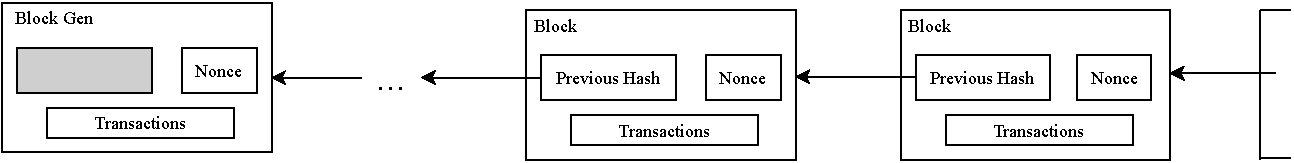
\includegraphics[scale=0.7]{figures/abstract_chain.pdf}
	\end{center}
	\caption{A high-level representation of a blockchain.}
	\label{fig:abstract_chain}
\end{figure}


Consider a peer-to-peer network where each party may have one of the following three roles:
lightweight \textit{clients}, full \textit{nodes} and \textit{miners}.
Miners maintain an updated copy of the chain locally, while providing computational power, also
called hashpower, to extend it. In order to extend the chain by one block, the miner has to perform
a proof-of-work as already described.
Full nodes can be thought of as miners with zero hashpower. Full nodes are also called
\textit{provers}, since they provide proofs  answering the queries for specific chain information
made by lightweight clients, according to Simplified Payment Verification (SPV) described by
Nakamoto\cite{nakamoto}.

According to SPV scheme lightweight clients only need to store the block headers of the longest
valid chain. A block header includes only a Merkle Tree Root of the Merkle Tree comprised by
the transactions included in that specific block. In order to validate that a transaction is
finalized, a client needs to query the nodes until he is convinced that he has the longest
valid chain, search for the block containing that transaction and finally verify an inclusion
proof of the transaction in the block of interest.

\begin{figure}[h!]
	\begin{center}
		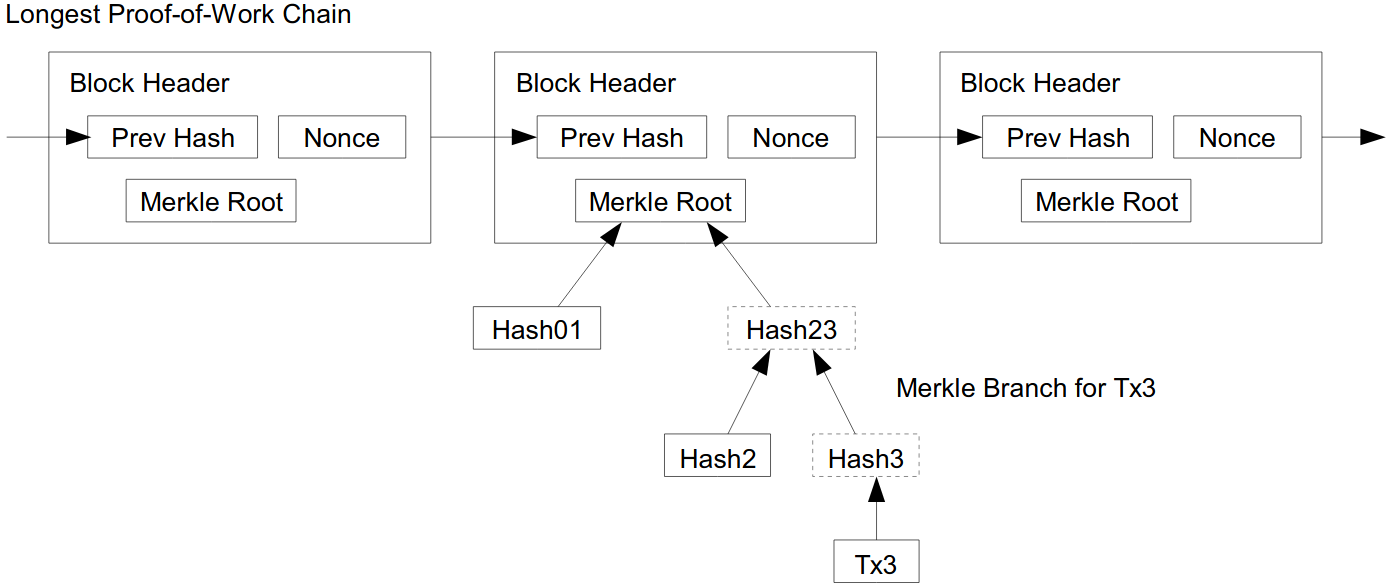
\includegraphics[scale=0.3]{figures/SPV_nakamoto.png}
	\end{center}
	\caption{High level representation of blockchain data kept by a lightweight client
	 and an inclusion proof for a transaction Tx3.\cite{nakamoto}}
	\label{fig:SPV_nakamoto}
\end{figure}

In the SPV scheme a client needs to store blockchain data of linear size to the whole chain. By
the time of writing Bitcoin's blockchain counts to almost 264GB and is estimated to grow more
than 50GB per year.  Since the growth rate of the chain is rather linear and constant, we need
to construct more efficient protocols serving the needs of lightweight clients. To this end,
the interaction between lightweight clients and full nodes is in our case supported  by the
NIPoPoWs\cite{nipopows} primitive which allows polylogarithmic poofs to the size of the chain.

\section{The Backbone Model}
The Backbone protocol is executed by an arbitrary number of parties over an unauthenticated network.
We consider $n$ parties in total, $t$ of which may be controlled by an adversary.

Table \ref{table:backbone_parameters} contains all the parameters of the Backbone protocol and will
be a point of reference throughout this work.

\begin{table}[h!]
	\begin{tabular}{| p{14.74cm} |}
		\hline
		$\lambda : \text{security parameter}$\\
		$\kappa : \text{length of the hash function output}$\\
		$n : \text{number of parties mining, } t \text{ of which are controlled by the adversary}$\\
		$T : \text{the target hash value used by parties for solving POW}$\\
		$t :  \text{number of parties controlled by the adversary}$\\
		$\delta : \text{advantage of honest parties}, \dfrac{t}{n-t} \leq 1-\delta$\\
		$f : \text{probability at least one honest party succeeds in finding a POW in a round}$\\
		$\epsilon : \text{random variables' quality of concentration in typical executions}$\\
		$k : \text{number of (suffix) blocks for the common prefix property}$\\
		% be more specific in l please\\
		$l : \text{number of blocks for the chain quality property}$\\
		$\mu_Q : \text{chain quality parameter}$\\
		%% more specific for s too please
		$s : \text{number of rounds for the chain growth property}$\\
		$\tau : \text{chain growth parameter}$\\
		$L : \text{the total run-tiem of the system}$\\
		\hline
	\end{tabular}
	\caption{The parameters of backbone model analysis. Positive integers $n, t, L, s, l, T, k,
	 \kappa$, positive reals $f, \epsilon, \delta, \mu_Q, \tau, \lambda$ where
	 $f, \epsilon, \delta, \mu_Q \in (0,1)$.}
	\label{table:backbone_parameters}
\end{table}

We will now give a high-level description of the Backbone Protocol and its fundamental components,
namely the three supporting algorithms for \textit{chain validation}, \textit{chain comparison} and
\textit{proof of work}. We will also define and discuss the three properties of the protocol, namely
\textit{Common Prefix}, \textit{Chain Quality} and \textit{Chain Growth}. For a more formal and
detailed presentation refer to the Backbone paper\cite{backbone}.

Consider that the protocol has already run for some rounds and a chain $C$ has been formed. Consider
also an honest party that wishes to connect to the network, obtain the up-to-date version of the
chain and try to extend it.
The honest party connects to the network and first tries to synchronize to the current chain. The
chain synchronization takes two steps to conclude. First, the newly connected peer receives a number
of candidate chains by other peers in the network and validates them one by one as for the structural 
properties of each block \textit{(Chain Validation)}. In particular, for each block the chain
validation algorithm checks that the proof-of-work is properly solved, that the hash of the previous
block is properly included in the block and that the the rest of the information included satisfies
a certain validity predicate $V(\cdot)$ depending on the application. For example, in Bitcoin
application it is checked that all the included transactions are valid according to the
UTXO set.

Afterwards, the \textit{Chain Comparison} algorithm is applied, where all the valid chains are
compared to each other and the longest one, as for total number of blocks or total hashing power
included, is considered the current active chain.

At last, in order to expand the chain by appending one more block to it, the \textit{Proof Of Work}
algorithm is applied, where the miner attempts to solve a proof of work as follows. The miner
constructs the contents of the block, including the hash of the previous block and a number of new
transactions published to the network. Consider that he can calculate the value $h = G(s,x)$ up
to this point. Finally it remains to compute the \textit{ctr} value so that $H(ctr, h) < T$. The
protocol is running in rounds and each party can make at most $q$ queries to function $H(\cdot)$
within a single round. If a suitable \textit{ctr} is found, an honest party quits any queries
remaining and announces the new born block to the network.

We can now define the three desired properties of the backbone protocol.\\
\begin{definition}[Common Prefix Property]
	The common prefix property $Q_{cp}$ with parameter
$k \in \mathbb{N}$ states that for any pair of honest players $P_1, P_2$ adopting the chains
$C_1, C_2$ at rounds $r_1 \leq r_2$ respectively, it holds that $C_1^{\lceil k} \preceq C_2$.
	\label{defn:common_prefix}
\end{definition}


\begin{definition}[Chain Quality Property]
	The chain quality property $Q_{cq}$ with parameters $\mu_{cq} \in \mathbb{R}$ and $l \in \mathbb{N}$ states that for any honest party $P$ with chain $\mathcal{C}$ it holds that for any $l $ consecutive blocks of $\mathcal{C}$ the ratio of honest blocks is at least $\mu_{cq}$.
	\label{defn:chain_quality}
\end{definition}

\begin{definition}[Chain Growth Property]
	The chain growth property $Q_{cg}$ with
parameters $\tau \in \mathbb{R}$ and $s \in \mathbb{N}$ states that for any honest party
\textit{P} with chain $\mathcal{C}$, it holds that for any $s$ rounds there are at least 
$\tau \cdot s$ blocks added to the chain of \textit{P}.
	\label{defn:chain_growth}
\end{definition}

\section{Hard, Soft and Velvet Forks}
We typically describe the two common types of a blockchain permanent fork as follows.

A \textit{hard fork} is a consensus protocol upgrade which is not backwards
compatible. This means that the changes in the protocol break the old rules
since the block header's contents change. After a hard fork blocks generated
by upgraded players are not accepted by the unupgraded ones. In order the
protocol update to be well established, the majority of the players must be
upgraded at an early point or else the non-upgraded players may maintain the
longest chain under the old rules.

A \textit{soft fork} is a consensus protocol upgrade which is backwards compatible.
This is usually implemented by keeping the old rules while adding additional
information in a way that unupgraded players can ignore as comments, for example,
by adding adding data in the coinbase transaction. In this way unupgraded players
accept blocks generated by upgraded miners as valid, while, typically, unupgraded
blocks are not accepted by upgraded players. Players are motivated to upgrade in
order their blocks to be accepted in the chain as valid.

A \textit{velvet fork} is also a backwards compatible consensus protocol upgrade.
Similar to soft fork additional data can be inserted in the coinbase transaction.
A velvet fork requires any block compliant to the old protocol rules only to be
accepted as valid by both unupgraded and upgraded players. By requiring upgraded
miners to accept all blocks, even if they contain false data according to the new
protocol rules, we do not modify the set of accepted blocks. Therefore, the upgrade
is rather a \textit{recommendation} and not an actual change of the consensus
protocol.  In reality, the blockchain is never forked. Only the codebase is
upgraded and the data on the blockchain is interpreted differently\cite{nipopows}.

The goal of this work is to provide a modified NIPoPoWs protocol so that it can be
deployed under a velvet fork in a provably secure manner.